\chapter{Resultados y Evaluación}
\label{cap:ResultadosYEvaluacion}

En este capítulo se muestran las pruebas realizadas sobre el modelo. El objetivo es el de evaluar el rendimiento del sistema y experimentar en el uso de las
diferentes combinaciones de espectrogramas, arquitecturas y funciones de pérdida para así obtener los mejores resultados posibles. Para ello, la fase se divide en dos vertientes:
evaluación sobre \textit{Test Set} y evaluación sobre \textit{Benchmark}. 

En la primera, se utilizan las muestras reservadas en la división inicial del dataset (un 15\%).
Los índices exactos de dicha muestra, se obtienen del archivo de punto de control (\textit{checkpoint}). 

En cuanto a la evaluación sobre \textit{Benchmark}, su objetivo 
es poner a prueba el manejo del modelo dada la característica no inyectividad de la síntesis FM. Para
ello, se diseña un banco de pruebas (\textit{benchmark}) con 12 sonidos de referencia que abarcan espacio tímbrico representativo
del sintetizador (desde un bajo limpio a sonidos agudos, complejos y muy ruidosos).

Sobre los resultados obtenidos por las dos vertientes previas, se pueden calcular diferentes métricas
para la evaluación del modelo en ambos ámbitos:

\begin{itemize}

\item \textbf{Métricas Sobre Parámetros: } Estas evalúan el modelo en función de la precisión obtenida
en los parámetros inferidos. Se emplean las métricas de: error cuadrático medio (MSE), que penaliza las desviaciones paramétricas grandes 
entre predicción y original; raíz del error cuadrático medio (RMSE), que devuelve el error en las unidades originales de cada parámetro, consiguiendo
ver de forma directa la precisión y así poder hacer comparaciones objetivas entre las distintas arquitecturas y funciones de pérdida;
y error absoluto medio (MAE), el cual es más robusto frente a valores atípicos. Estas métricas sufren ante el problema de la no inyectividad 
, por lo que se utilizan principalmente como diagnóstico rápido.

\item \textbf{Métricas de Audio: } Estas son mucho más interesantes para conseguir una evaluación
similar a la que daría un oído experto, ya que se usan para sintetizar sonidos con los parámetros obtenidos y realizan una comparativa
perceptual de los sonidos. Primero se aplica la Distancia L1 en Espectrogramas Mel (\textit{Mel l1}), la cual calcula el 
Error Absoluto Medio (L1) sobre las señales previamente transformadas a la escala Mel, consiguiendo así la sensibilidad logarítmica
del oído humano. De igual manera se aplica la Distorsión Cepstral Mel (MCD - \textit{Mel-Cepstral Distortion}). Es una métrica que trata 
de evaluar la similitud del timbre de los audios, extrayendo 13 Coeficientes Cepstrales en las Frecuencias de Mel (MFCC). 
El primer coeficiente, que representa la energía global, es descartado para que la métrica refleje exclusivamente el timbre (textura del sonido).

\item \textbf{Métrica de Reconstrucción (Decoder L1): } En el caso en el que se utilice la arquitectura
\textbf{CNNRegressor5}. Calcula el Error Absoluto Medio (L1) entre el espectrograma original y el reconstruido por la red,
de forma que se consigue evaluar la asimilación de información en el espacio latente. 

\end{itemize} 

\section{Definición de los Pipelines Experimentales}

\begin{figure}[H] 
    \centering
    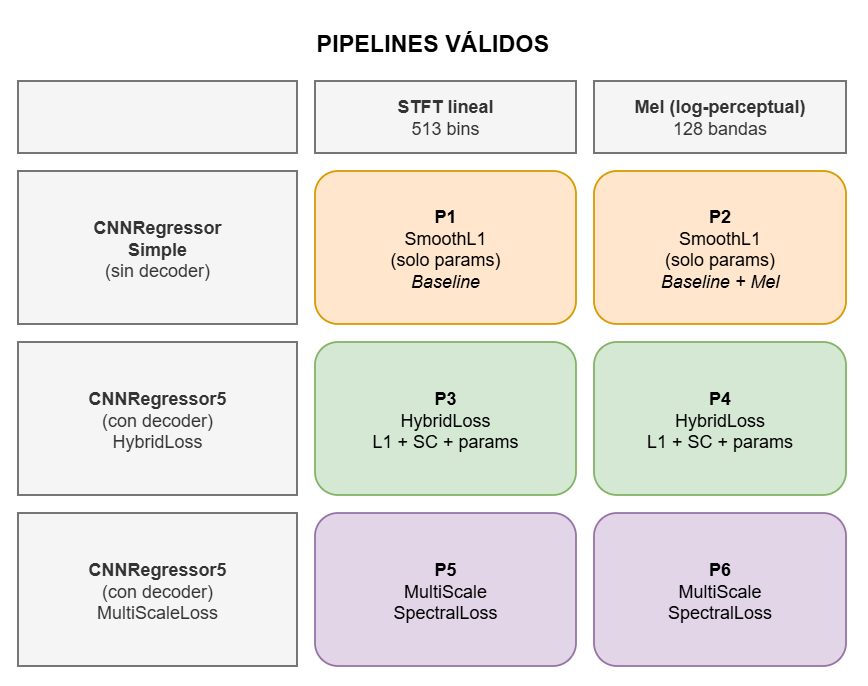
\includegraphics[width=1\textwidth]{Imagenes/Bitmap/pipelines}
    \caption{Representación de las diferentes combinaciones de Arquitecturas y Funciones de Pérdida.}
    \label{fig:pipelines}
\end{figure}

La Figura \ref{fig:pipelines} muestra las diferentes configuraciones que se dan combinando las arquitecturas y funciones de pérdida previamente definidas.

\section{Introduccion y Configuración del Entorno}

\subsection{Características del \textit{Hardware} empleado en el entrenamiento de los modelos}

Para la contextualización de los datos de tiempos requeridos en el entrenamiento de los diferente modelos, se especifican las características de las máquinas empleadas:
\noindent \textbf{\textit{GPUs}:}
\begin{itemize}
    \item \textbf{Máquina Cedida por la Universidad: }NVIDIA GeForce RTX 3070
    \item \textbf{Ordenador Personal David: }NVIDIA GeForce RTX 3050 
\end{itemize}

%En cada apartado se especifica la máquina utilizada para su entrenamiento.

%(TODO) Insertar tabla con las características

\subsection{Configuración de las Pruebas}
La evaluación de las topologías se ha llevado a cabo con un único dataset de 50000 audios (método de generación explicado aquí: \ref{sec:GeneracionDataset}), un número que ha resultado ser equilibrado, perimitiendo unos resultados decentes sin suponer un incremento demasiado grande en los tiempos de entrenamiento de los modelos. 

El número de épocas no se ha mantenido fijo, se ha utilizado un valor de paciencia (\textit{Early Stopping}) de 10 épocas. De esta manera, se comprueba el error de validación en cada época y si despues de 10 seguidas no se ha mejorado su record histórico, la red deja de entrenarse. Así pues, se evita la sobreadaptación (\textit{overfitting}) de la red neuronal, puesto que se evita un entrenamiento excesivo, y se ahorra tiempo. 

Por otro lado, se ha elegido un \textit{Batch Size} de tamaño 32. Este, aparte de ser un estándar, es un valor asumible por cualquier tarjeta gráfica moderna y que consigue una eficiencia adecuada. 

\noindent \textbf{\textit{Benchmark}:}
\begin{itemize}
    \item \textbf{Tamaño del Dataset: }50000
    \item \textbf{Valor de Paciencia: }10 
    \item \textbf{\textit{Batch Size}: }32
\end{itemize}

\subsection{Convergencia y Dinámica del Entrenamiento}

\begin{table}[H]
    \centering
    \renewcommand{\arraystretch}{1.2}
    \begin{tabular}{|c|c|c|c|}
    \hline
    \textbf{Modelo} & \textbf{Función de Pérdida (Validación)} & \textbf{Épocas} & \textbf{Error de Validación (Mínimo)} \\ \hline\hline
    \textbf{P1} & SmoothL1 (Paramétrica) & 35 & 0.0159 \\ \hline
    \textbf{P2} & SmoothL1 (Paramétrica) & 57 & 0.0068 \\ \hline\hline
    \textbf{P3} & HybridLoss (Acústica) & 59 & 0.3830 \\ \hline
    \textbf{P4} & HybridLoss (Acústica) & 25 & 0.6723 \\ \hline\hline
    \textbf{P5} & MultiScaleSpectralLoss (Acústica) & 35 & 0.4297 \\ \hline
    \textbf{P6} & MultiScaleSpectralLoss (Acústica) & 60 & 0.6974 \\ \hline
    \end{tabular}
    \caption{Resumen del rendimiento durante la fase de entrenamiento (\textit{Early Stopping} = 10). Cabe destacar que los errores de los modelos que presentan funciones de pérdida diferentes no son comparables.}
    \label{tab:entrenamiento_epochs}
\end{table}

La Tabla \ref{tab:entrenamiento_epochs} muestra el funcionamiento de \textit{Early Stopping} y cómo cada red tarda un número diferente de épocas en llegar a cumplir con este valor de paciencia. Destaca en la eficiencia de entrenamiento el modelo P4, el cual consigue entrenarse en tan solo 25 \textit{epochs}, mientras que la arquitectura P3, que solo difiere en el tipo de espectrograma, necesitó extenderse hasta las 59 épocas. 

Es importante remarcar que los resultados de los errores de validación de diferentes funciones de pérdida no son comparables, siendo lógico que las pérdidas paramétricas registren errores inferiores en comparación a las pérdidas acústicas, ya que estas miden diferencias de magnitud y energía (en decibelios).

\subsection{Análisis Crítico de las Métricas de Evaluación}
\label{sec:AnalisisCriticoMetricas}
Antes de continuar con las preubas detalladas de los modelos y su análisis, es importante mencionar un sesgo en el cálculo de las métricas acústicas de error.

Durante la experimentación, se dectectó una relación directa entre la duración del sonido de los audios y la puntuación obtenida sobre las métricas. En el caso de Mel L1, se calcula el error medio durante el total de la extensión de la muestra (fijada en 2 segundos) y como los modelos predicen con mucha precisión los silencios, los audios que contienen una parte considerable sin sonido consiguen puntuaciones mejores.

A pesar de este hecho, la experimentación no queda invalidada, simplemente se tiene en cuenta para la interpretación de las gráficas.

\section{Evaluación sobre el Conjunto de Prueba (\textit{Test Set})}

\begin{figure}[H]
    \centering
    
    % --- FILA 1: P1 y P2 ---
    \begin{subfigure}[b]{0.48\textwidth}
        \centering
        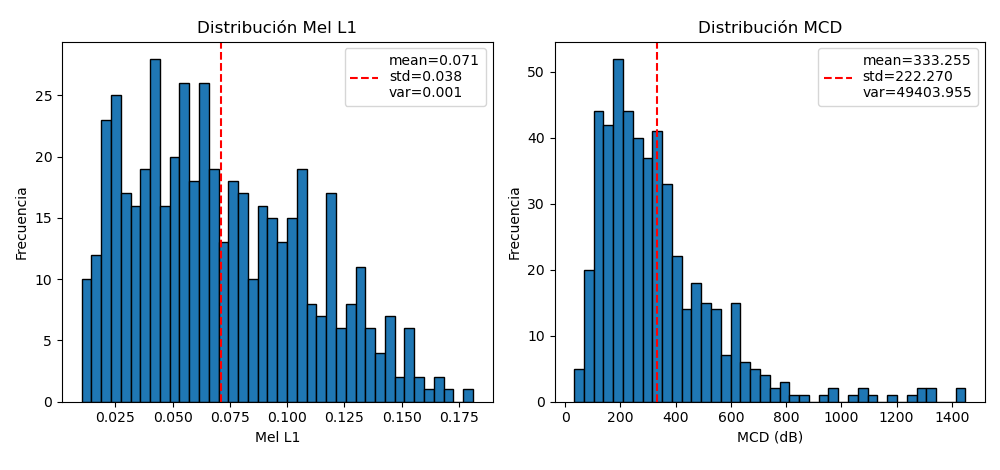
\includegraphics[width=\textwidth]{Imagenes/Bitmap/test_set_p1}
        \caption{Modelo P1 (STFT Lineal - SmoothL1)}
        \label{fig:sub_test_p1}
    \end{subfigure}
    \hfill
    \begin{subfigure}[b]{0.48\textwidth}
        \centering
        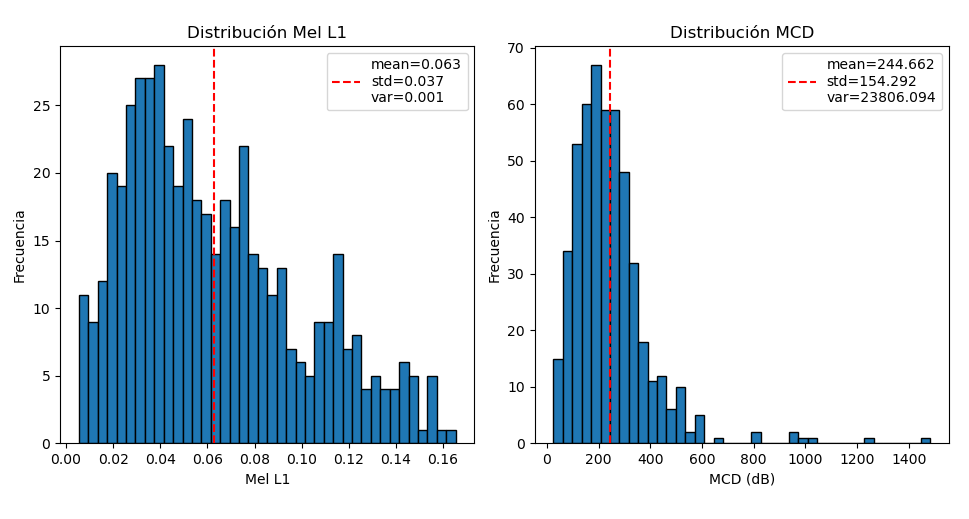
\includegraphics[width=\textwidth]{Imagenes/Bitmap/test_set_p2}
        \caption{Modelo P2 (Mel log-perceptual - SmoothL1)}
        \label{fig:sub_test_p2}
    \end{subfigure}
    
    \vspace{0.4cm} % Espacio vertical entre la fila 1 y la fila 2
    
    % --- FILA 2: P3 y P4 ---
    \begin{subfigure}[b]{0.48\textwidth}
        \centering
        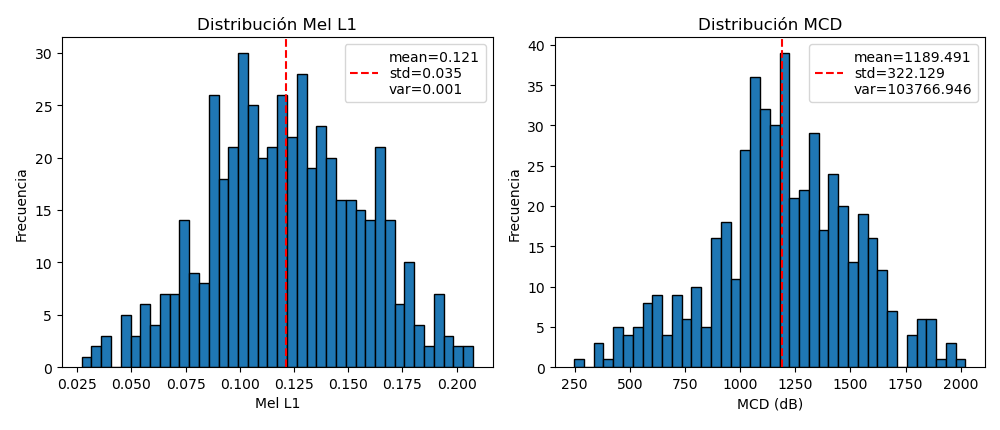
\includegraphics[width=\textwidth]{Imagenes/Bitmap/test_set_p3}
        \caption{Modelo P3 (STFT Lineal - HybridLoss)}
        \label{fig:sub_test_p3}
    \end{subfigure}
    \hfill
    \begin{subfigure}[b]{0.48\textwidth}
        \centering
        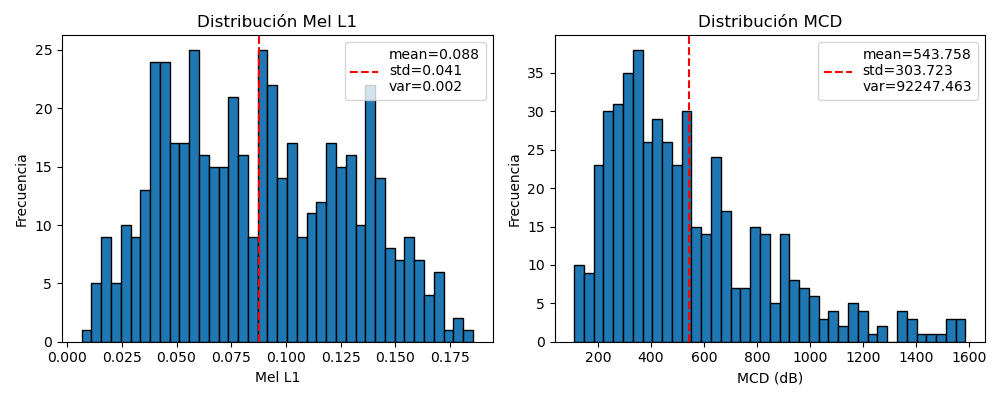
\includegraphics[width=\textwidth]{Imagenes/Bitmap/test_set_p4}
        \caption{Modelo P4 (Mel log-perceptual - HybridLoss)}
        \label{fig:sub_test_p4}
    \end{subfigure}

    \vspace{0.4cm} % Espacio vertical entre la fila 2 y la fila 3

    % --- FILA 3: P5 y P6 ---
    \begin{subfigure}[b]{0.48\textwidth}
        \centering
        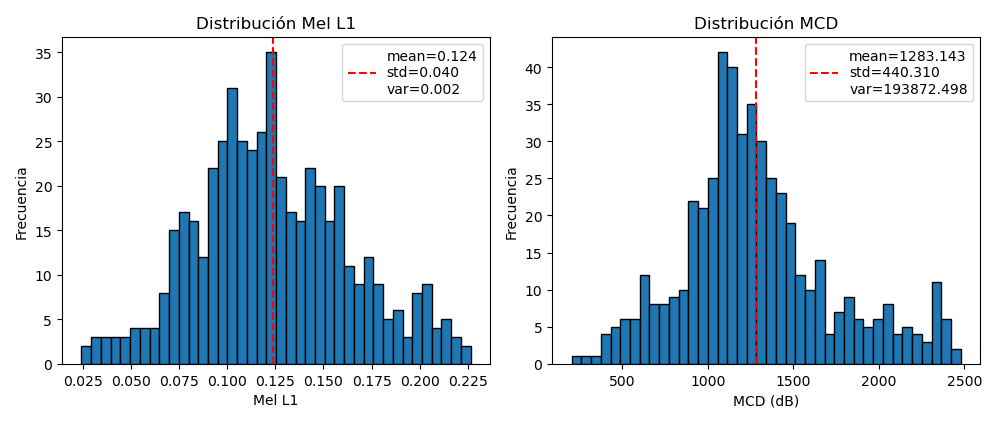
\includegraphics[width=\textwidth]{Imagenes/Bitmap/test_set_p5}
        \caption{Modelo P5 (STFT Lineal - MultiScale)}
        \label{fig:sub_test_p5}
    \end{subfigure}
    \hfill
    \begin{subfigure}[b]{0.48\textwidth}
        \centering
        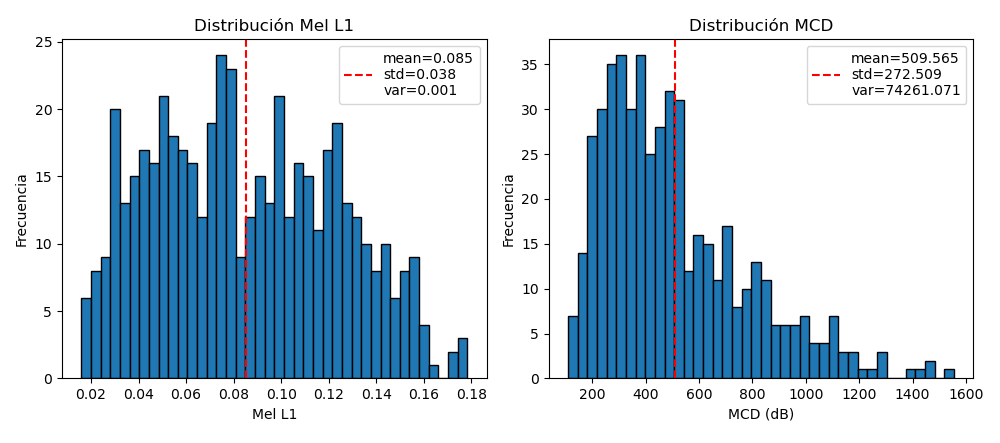
\includegraphics[width=\textwidth]{Imagenes/Bitmap/test_set_p6}
        \caption{Modelo P6 (Mel log-perceptual - MultiScale)}
        \label{fig:sub_test_p6}
    \end{subfigure}

    \caption{Comparativa global de la dispersión de las métricas Mel L1 y MCD en el Test Set para los seis pipelines experimentales.}
    \label{fig:comparativa_test_set_global}
\end{figure}

\begin{table}[H]
    \centering
    \renewcommand{\arraystretch}{1.3} % Da un poco de aire vertical a las celdas
    \begin{tabular}{|c||c|c|}
    \hline
    \textbf{Pipeline} & \textbf{Mel L1 (dB) $\downarrow$} & \textbf{MCD $\downarrow$} \\ \hline\hline
    \textbf{P1} & $0.071 \pm \text{0.038}$ & $333.255 \pm \text{222.270}$ \\ \hline
    \textbf{P2} & $0.063 \pm 0.037$ & $244.662 \pm 154.292$ \\ \hline
    \textbf{P3} & $0.121 \pm \text{0.035}$ & $1189.491 \pm \text{322.129}$ \\ \hline
    \textbf{P4} & $0.088 \pm \text{0.041}$ & $543.758 \pm \text{303.723}$ \\ \hline
    \textbf{P5} & $0.124 \pm \text{0.040}$ & $1283.143 \pm \text{440.310}$ \\ \hline
    \textbf{P6} & $0.085 \pm \text{0.038}$ & $509.565 \pm \text{272.509}$ \\ \hline
    \end{tabular}
    \caption{Resultados (Media $\pm$ Desviación Estándar) de las métricas acústicas sobre el \textit{Test Set} para las seis topologías.}
    \label{tab:metricas_exactas_test}
\end{table}

La Figura \ref{fig:comparativa_test_set_global} recoge la distribución visual de los errores de cada arquitectura, marcando dónde se encuentra la media. Por otro lado, la Tabla \ref{tab:metricas_exactas_test} contiene la información exacta de la media y desviación estándar de cada modelo.

Al proceder con la comparación de cada modelo con su contraparte con la misma arquitectura y diferente tipo de espectrograma, se puede apreciar que los modelos con espectrogramas Mel han conseguido resultados que superan significativamente a los obtenidos con STFT. Como indican los datos, P2 consigue errores inferiores a P1, P4 a P3 y P6 a P5. 

Este resultado era esperable, debido a la característica ya comentada de los espectrogramas Mel, que simulan la percepción del oído humano y facilitan la extracción de características a la red neuronal. 

En cuanto al mejor resultado obtenido en la evaluación del conjunto de prueba, sorprende que se trate de P2, puesto que su función de pérdida (\textit{SmoothL1}) es paramétrica, lo cual hemos visto con anterioridad que es arriesgado porque la síntesis FM no es inyectiva y las funciones híbridas (de P3 a P6) surgían del intento de asumir dicha característica. Adicionalmente, cabe destacar que P2 utiliza la arquitectura \textit{CNNRegressorSimple}, de la cual, al ser más simple y carecer de \textit{decoder}, se esperaban peores resultados.

El análisis de los resultados no nos lleva a descartar directamente los últimos modelos y a quedarnos únicamente con P2, sino que encontramos una explicación que justifica los resultados. Las estructuras simples presentan una ventaja inicial en este caso: para la red resulta considerablemente más sencillo comparar números exactos en funciFones de pérdida paramétricas que evaluar imágenes (espectrogramas) en funciones acústicas.

Al añadir un \textit{decoder} y funciones de pérdida acústicas e híbridas, es muy probable que se trate de arquitecturas muy complejas para el tamaño del dataset. En consecuencia, la red neuronal se centra también en la reconstrucción de los detalles visuales en lugar de exclusivamente en aprender los parámetros. 

%Estoy pensando en mover esto a un apartado final de conclusiones del capítulo
Como conclusión, queda claro que para el tamaño de dataset limitado que hemos utilizado, los modelos simples convergen antes en mejores resultados, pero como línea de trabajo futuro interesaría ampliar los datos y seguir probando los modelos complejos.

En cuanto a la dispersión de los valores de cada modelo (véase Figura \ref{fig:comparativa_test_set_global} y la Tabla \ref{tab:metricas_exactas_test}), se puede apreciar que la dispersión de los modelos es, en general, elevada, sobre todo en modelos como P1 y P2 con desviaciones estándar en la métrica MCD que se acercan considerablemente a la media. En Mel L1 se suelen presentar valores que no se alejan mucho de la media pero los valores que se alejan tienen frecuencias de aparición altas, subiendo  así la desviación estándar. En cuanto a MCD, la mayoría de los valores se congregan alrededor de la media, pero existen unos pocos casos con resultados muy alejados que sesgan la desviación estándar. 

Para entender la escasez de consistencia de los modelos y los casos que se salen de los valores de las medios de las métricas, hace falta tener en cuenta el sesgo de Mel L1 y MCD (véase \ref{sec:AnalisisCriticoMetricas}). En la Figura \ref{fig:comparativa_test_set_global}, los valores de las gráficas que más se alejan de la media, es muy probable que sean audios cortos/percusivos (los que consiguen mejor puntuación) y largos/sostenidos (los que más se alejan por la derecha).

Para comprobar esta hipótesis, en la siguiente sección se analiza cómo cada red gestiona distintos tipos de audio.



\section{Evaluación sobre el Banco de Pruebas (\textit{benchmark})}

\begin{figure}[H]
    \centering
    
    % --- FILA 1: P1 y P2 ---
    \begin{subfigure}[b]{0.48\textwidth}
        \centering
        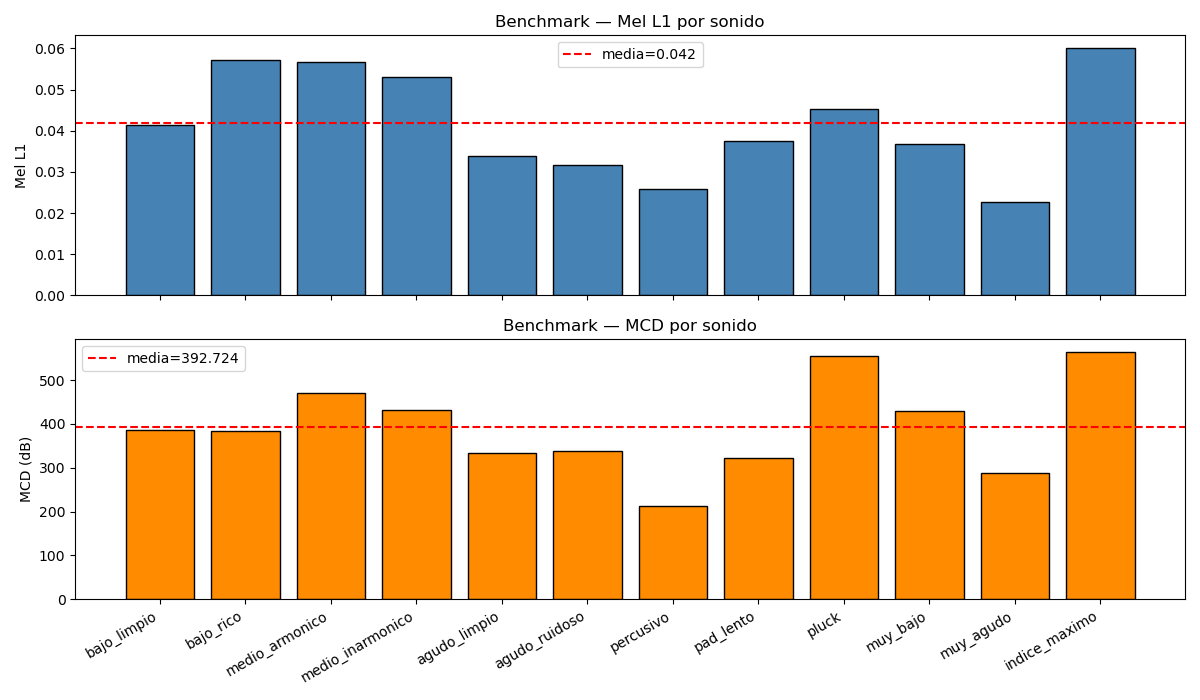
\includegraphics[width=\textwidth]{Imagenes/Bitmap/benchmark_P1}
        \caption{Modelo P1 (STFT Lineal - SmoothL1)}
        \label{fig:sub_bench_p1}
    \end{subfigure}
    \hfill
    \begin{subfigure}[b]{0.48\textwidth}
        \centering
        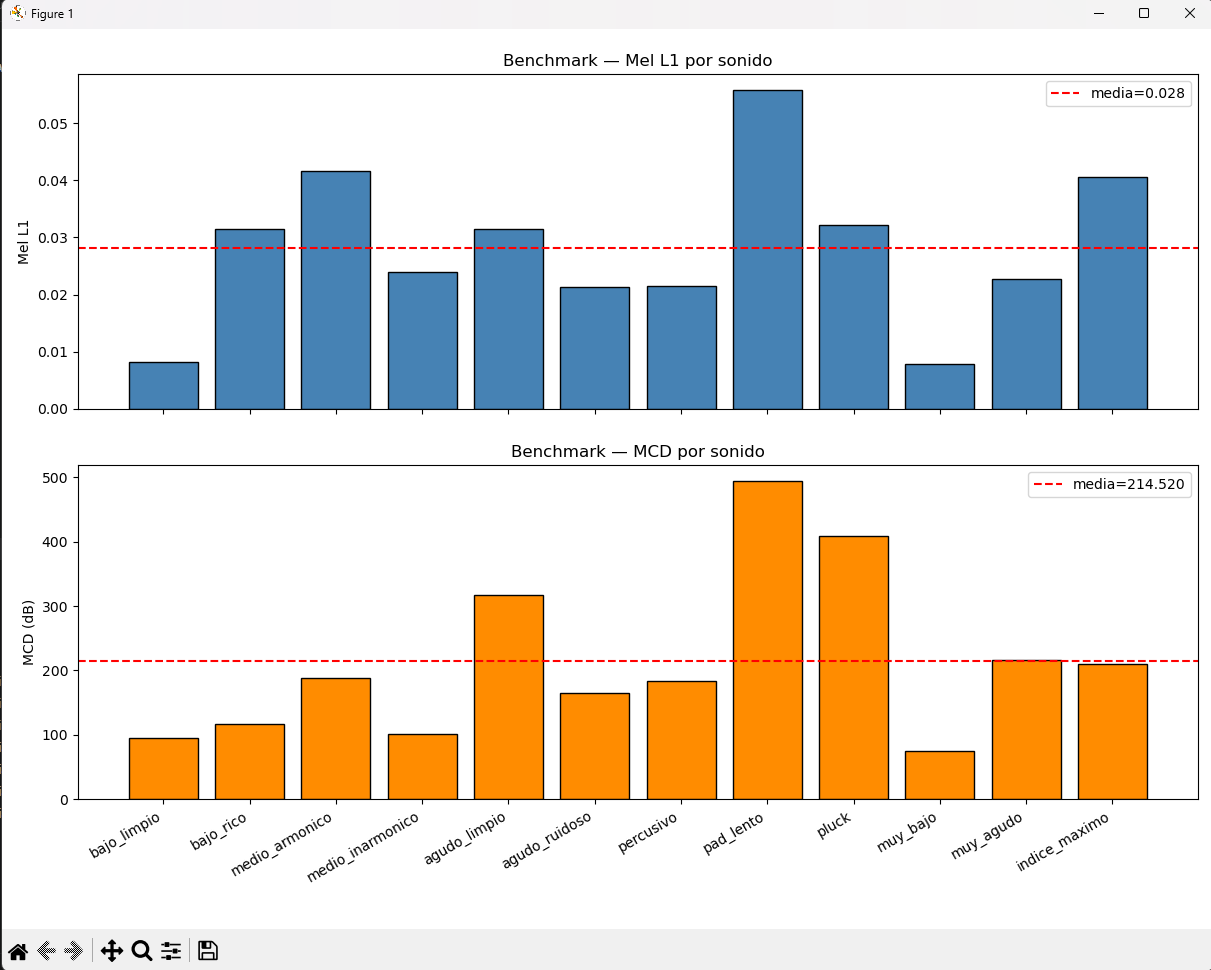
\includegraphics[width=\textwidth]{Imagenes/Bitmap/benchmark_P2}
        \caption{Modelo P2 (Mel log-perceptual - SmoothL1)}
        \label{fig:sub_bench_p2}
    \end{subfigure}
    
    \vspace{0.4cm} 
    
    % --- FILA 2: P3 y P4 ---
    \begin{subfigure}[b]{0.48\textwidth}
        \centering
        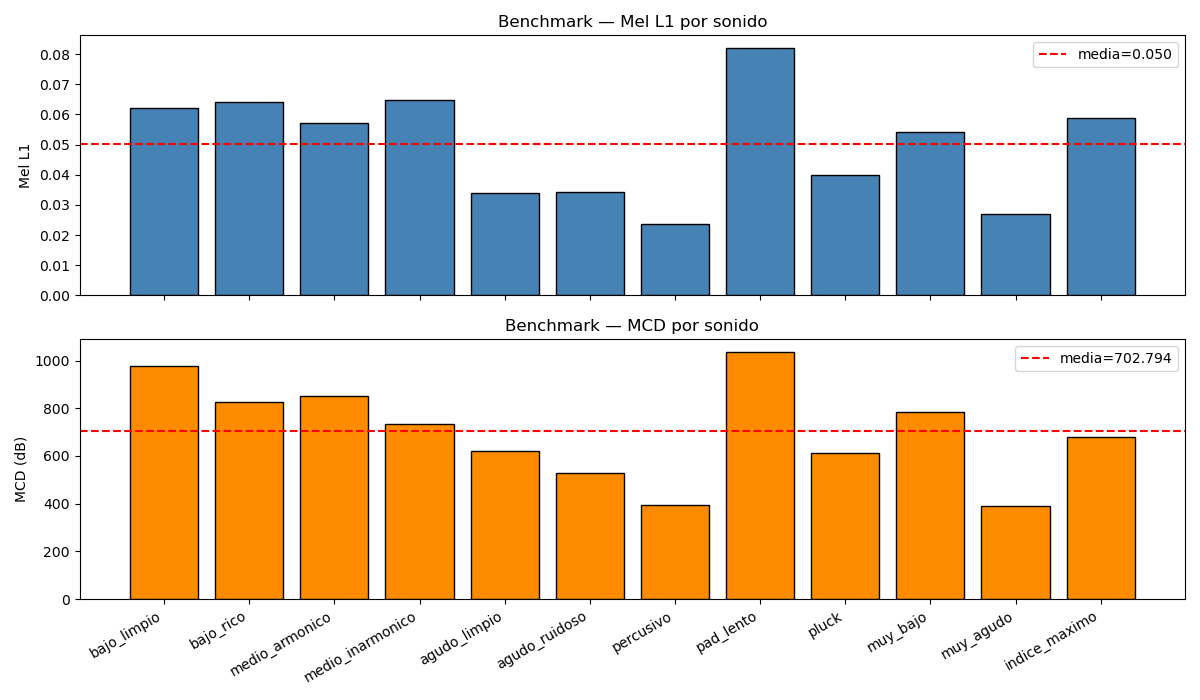
\includegraphics[width=\textwidth]{Imagenes/Bitmap/benchmark_P3}
        \caption{Modelo P3 (STFT Lineal - HybridLoss)}
        \label{fig:sub_bench_p3}
    \end{subfigure}
    \hfill
    \begin{subfigure}[b]{0.48\textwidth}
        \centering
        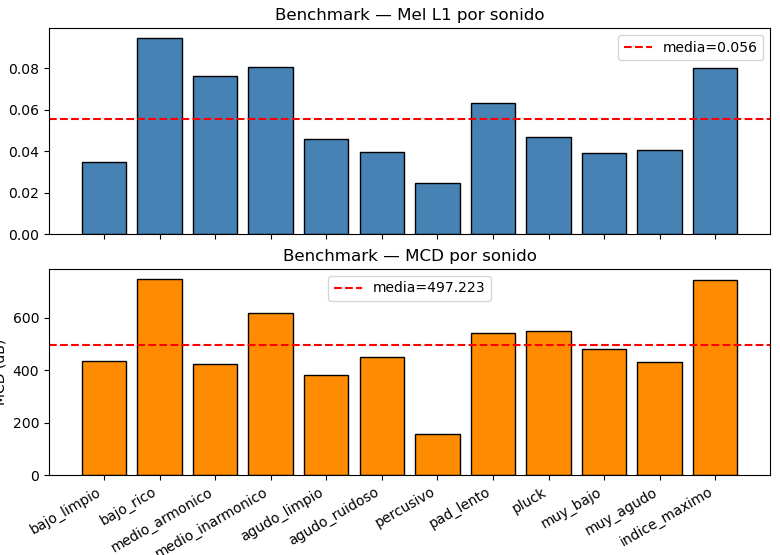
\includegraphics[width=\textwidth]{Imagenes/Bitmap/benchmark_P4}
        \caption{Modelo P4 (Mel log-perceptual - HybridLoss)}
        \label{fig:sub_bench_p4}
    \end{subfigure}

    \vspace{0.4cm} 

    % --- FILA 3: P5 y P6 ---
    \begin{subfigure}[b]{0.48\textwidth}
        \centering
        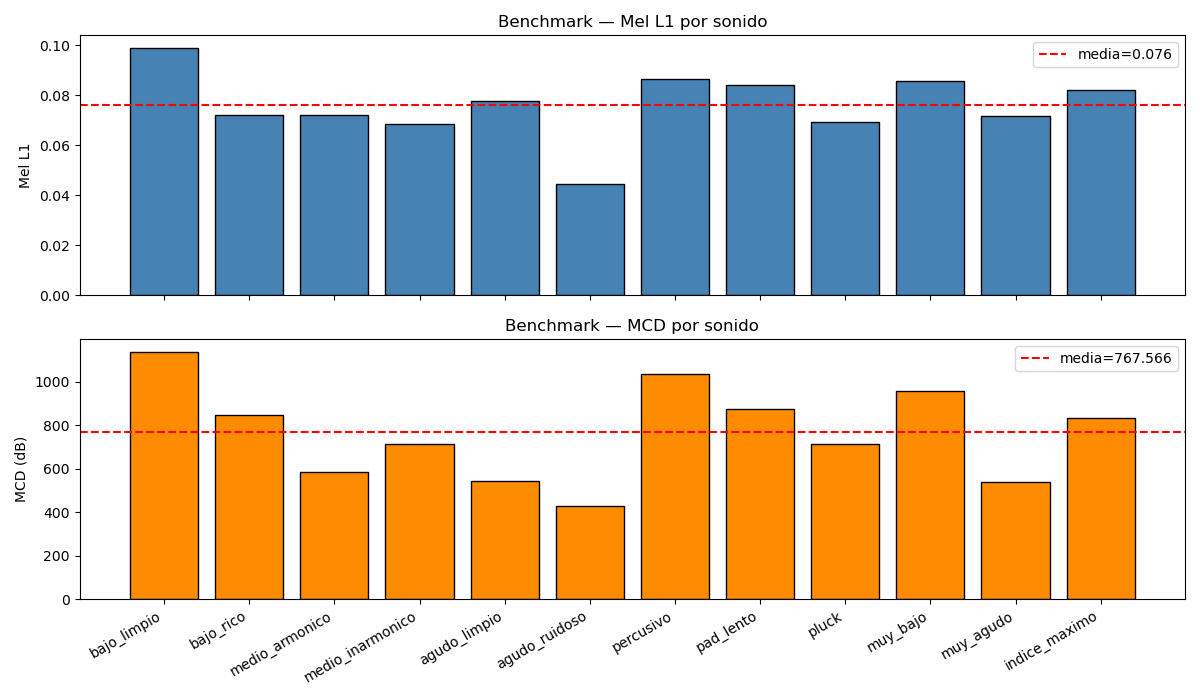
\includegraphics[width=\textwidth]{Imagenes/Bitmap/benchmark_P5}
        \caption{Modelo P5 (STFT Lineal - MultiScale)}
        \label{fig:sub_bench_p5}
    \end{subfigure}
    \hfill
    \begin{subfigure}[b]{0.48\textwidth}
        \centering
        \includegraphics[width=\textwidth]{Imagenes/Bitmap/benchmark_P6}
        \caption{Modelo P6 (Mel log-perceptual - MultiScale)}
        \label{fig:sub_bench_p6}
    \end{subfigure}

    \caption{Comparativa del rendimiento de los seis modelos sobre los 12 sonidos del \textit{benchmark}. Se evalúan las métricas Mel L1 y MCD. La media de cada una se marca con una línea roja. En el eje de horizontal se representan los distintos audios en el siguiente orden (de izquierda a derecha): 1) \textit{bajo\_limpio}, 2) \textit{bajo\_rico}, 3) \textit{medio\_armonico}, 4) \textit{medio\_inarmónico}, 5) \textit{agudo\_limpio}, 6) \textit{agudo\_ruidoso}, 7) \textit{percusivo}, 8) \textit{pad\_lento}, 9) \textit{pluck}, 10) \textit{muy\_bajo}, 11) \textit{muy\_agudo} y 12) \textit{indice\_maximo}.}
    \label{fig:comparativa_benchmark_global}
\end{figure}

\subsection{Comportamiento ante sonidos percusivos y cortos}

\subsection{Comportamiento ante sonidos graves y armónicos}

\subsection{Comportamiento ante sonidos sostenidos complejos}